\section{One finite start, accountable operation}
\label{sec:operations}

\subsection{The actual Alpha execution path}

Each mission uses the released Alpha v1.42.0 \artifact{createWorkbench} extension from source commit
\artifact{c352bad0a0941fdccd490a7224e3efd1b8de45d5} \citep{alphaWorkbench1420}.
The eight-file execution closure is unchanged; the current-main entry file is byte-identical to that release.
A ninth vendored file is the existing transactional browser history store, obtained at current-main commit
\artifact{5499495911bf8822ac0aa8c9007f00789c1132b5}. Its identity is recorded separately from the execution
closure. A persistent local Node bridge validates and freezes a request, invokes its registered local adapter, requests the
fixed Python callback, binds the returned artifact and inspects the original workbench pack. Numerical
computation therefore follows workbench dispatch. It is not computed first and retrospectively wrapped as
an agent result.

The concrete seam is \artifact{createWorkbench(adapters).run(spec, options)}, followed by
\artifact{inspectPack(pack)}. The Python client supplies mission identity, purpose, exact inputs, the fixed
callback and the enclosing source hash. The callback returns a finite report with validity, qualification
and measured output; it cannot confer the independent institutional proof that the upstream template lacks.

The finite research recipe supplies the declared mission sequence. It is not a newly installed scheduler.
The maintained native \artifact{CampaignOperation} uses the existing source-clause study queue and fixed
selectors; it does not offer this numerical family. The native workbench invokes its shipped fixed worker
families and local identity machinery. Neither path is silently substituted or initialized here. The preserved
research scheduler is another distinct implementation. A local workbench extension is useful executable
integration within its declared scope, not proof that an authenticated native service is operating.

\subsection{Service and improvement have separate accounts}

The custody layer maintains separately enforced service and improvement allowances. Earned capacity starts
at zero. Reservations name one account; failed research cannot borrow the service balance. Measured CPU is
settled in integer microseconds. Work beyond a reservation is recorded at its actual cost, refused and placed
on accounting HOLD. The accounting does not physically preempt an indivisible native numerical call.
Input-size/call bounds and observed overruns must therefore be reported honestly.

The frozen allowances per stream are 10,000\,ms of service-dispatch CPU, 1,000\,ms of external
improvement-dispatch CPU and a 500\,ms cumulative transfer cap. Each accepted B mission may release
50\,ms; the eight B missions can therefore release at most 400\,ms. Construction reserves
400\,ms and restoration 600\,ms. A separate 2,000\,ms external control allowance covers
shared startup, custody settlement and aggregate artifacts. The wall deadline is 300\,s and the
absolute local authority expiry 600\,s. Dispatch, control and total-process measures retain their
different boundaries; overlapping CPU measurements are not added twice.

Only a completed, accepted service request can release its unused reserved allowance into the earned account,
subject to a cumulative cap. That transfer conserves the original endowment. It creates no money and does not
itself prove that the capability saved compute: an overly generous reservation would also leave slack.
The scientific resource certificate must separately identify the matched alternative, measured incremental
benefit, available capacity and the subsequent construction that consumed it. Released external allowance and
improvement-earned capacity are distinct labels unless that evidence supports their equivalence.

\begin{figure}[ht]\centering
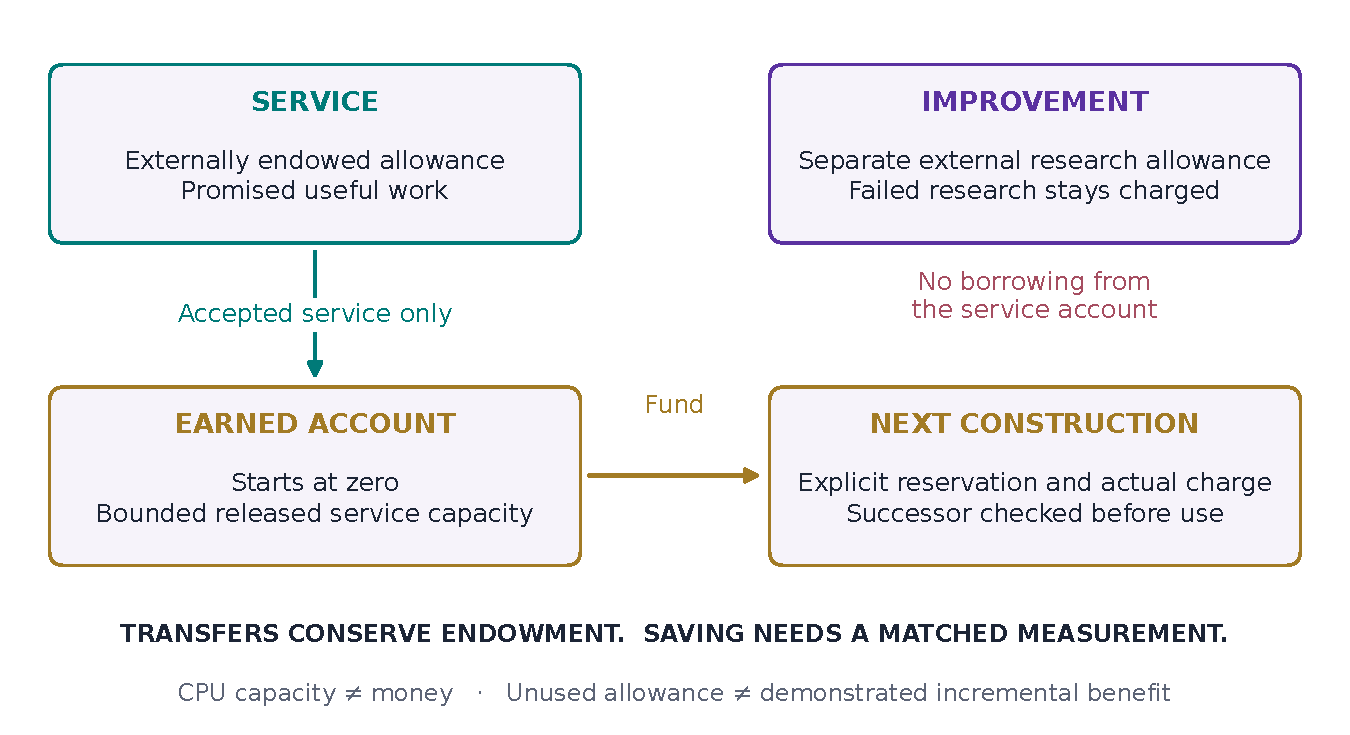
\includegraphics[width=\linewidth]{figures/resource-ledger.pdf}
\caption{Three accounts, two origins. Research has its own external allowance. Earned capacity begins empty and can receive a bounded transfer from accepted service. The transfer is conserved resource custody; evidence of incremental saving is a separate causal requirement. No CPU quantity is converted into cash.}
\label{fig:accounts}
\end{figure}

\subsection{Recovery preserves cost and refusal}

A single-writer local journal retains requests, receipts, account changes, stops and asset dispositions in a
contiguous hash chain with a separately appended head anchor. A completed duplicate returns the same receipt
without another execution instruction or charge. A pending reservation found after an interrupted process is
quarantined and conservatively charged its reserved ceiling; its true lost CPU remains unknown. The system
does not retry uncertain work under a fresh name and omit its cost.

Source or dependency changes, invalid receipts, stale checkpoints and exhausted allowances fail closed.
STOP persists across restart. Explicit resume retains the stop history and the original absolute expiry;
it cannot extend authority. A result arriving after STOP or expiry is retained for accounting but not accepted.
Rollback selects a still-applicable earlier asset without rewinding history. Rejected descendants cannot
re-enter through restored state, and a rejected parent invalidates dependent selection.

\paragraph{An actual process boundary.}
The frozen recovery probe uses the declared development network of 576 nodes, outside the efficacy
confirmation. Worker PID~7 dispatches and independently checks A, persists its portable factor and accepted
receipt, closes its Node bridge and exits with code~23 before acknowledgement. Worker PID~19 opens the same
custody directory: repeating A returns the original receipt with no second execution; a fresh B load uses the
restored factor through another workbench dispatch and passes the edge-based check. The retained execution
ledger contains exactly one A and one B. All ten probe checks pass, including unchanged parent identity and
empty inherited current proof and authority. Total worker-and-descendant CPU is 692.213\,ms; wall time
is 688.143\,ms. This intentional post-commit exit tests lost acknowledgement across OS processes, not
every possible crash window. Pending-commit quarantine is tested separately.

\begin{figure}[ht]\centering
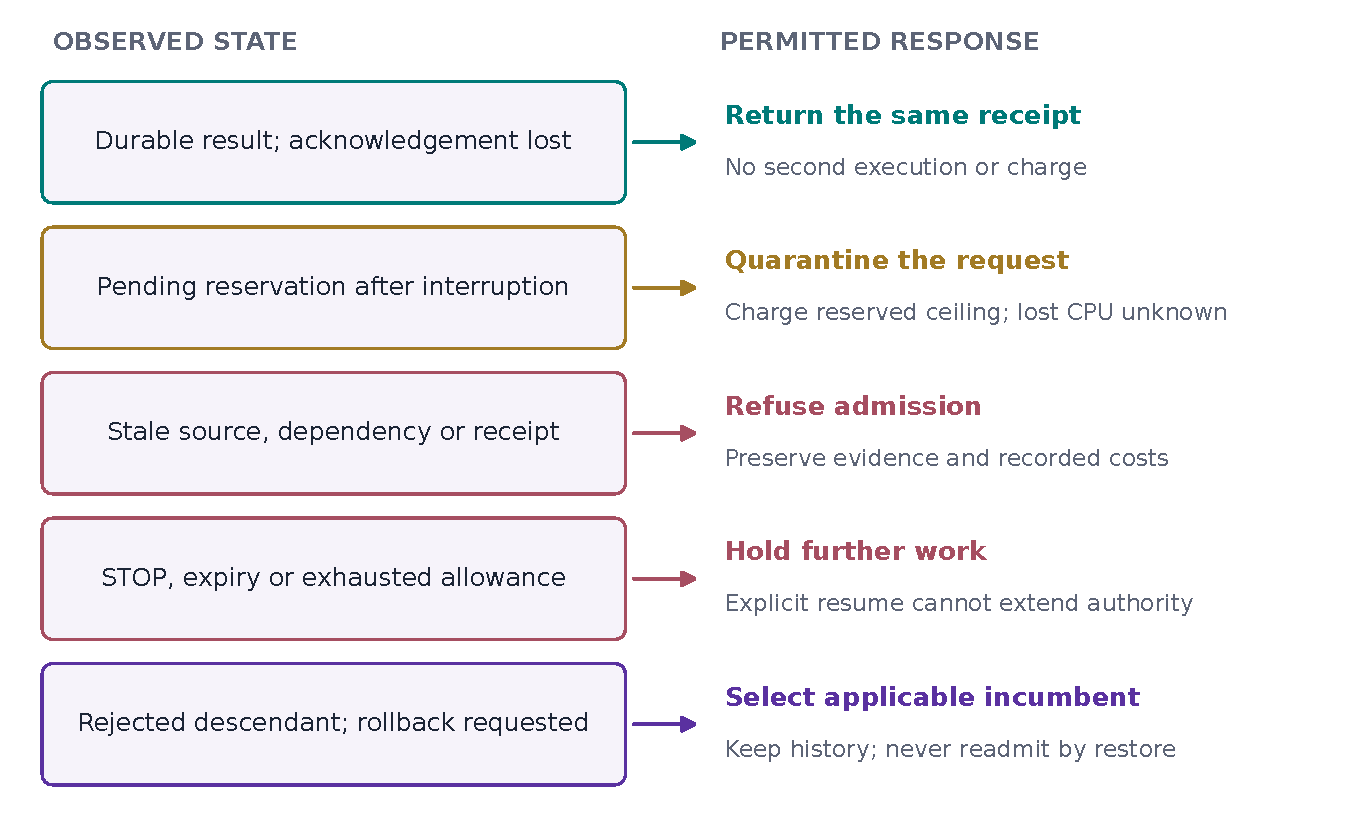
\includegraphics[width=\linewidth]{figures/failure-recovery-map.pdf}
\caption{Recovery preserves the distinction between completed, uncertain and forbidden work. A lost acknowledgement after durable commitment returns the original result; an unresolved reservation is conservatively charged and quarantined. Rejection, STOP and expiry cannot be cleared by replaying history. The map describes tested local controls, not an external exactly-once service guarantee.}
\label{fig:recovery}
\end{figure}

\begin{table}[ht]\centering\small
\begin{tabularx}{\linewidth}{L{36mm}L{17mm}Y}
\toprule
Evidence set & Outcome & Scope and relevant boundary \\
\midrule
Workbench bridge & 10/10 & Actual callback order; duplicate refusal; invalid source/receipt; callback failure; STOP before and after work. \\
Custody components & 16/16 & Journal, dependencies, distinct budgets, persistent STOP, expiry, rollback and pending quarantine. One expiry-during-work check injects a development clock. \\
Two OS processes & 10/10 & Durable A; deliberately lost acknowledgement; no duplicate A; portable parent used on fresh checked B. \\
Confirmation restoration & 42/42 & Six maintenance streams across seven arms; restored or rechecked methods produce qualified outputs. \\
Confirmation scope & 168/168 & One unsupported conductance case per stream and arm is refused; no unsupported solution enters qualified coverage. \\
Browser checker & 17/17 & Independent edge calculation and malformed input/output, changed dependency and ancestry checks. \\
Browser journey & 21/21 & Actual local computation, retained reference, downloads, mobile layout, STOP, resume and no outbound request. \\
Browser interruption & 8/8 & Real page reload with a pending reservation, conservative charge, durable-boundary resume and corrupted-state refusal. \\
\bottomrule
\end{tabularx}
\caption{Separate operational evidence sets. These counts are checks or stream events, not independent efficacy samples. Component and browser records are development evidence; the OS probe executes the final frozen source on development inputs.}
\label{tab:operationchecks}
\end{table}

These are local integrity controls. The unsigned journal and anchor share one host; replacing both with an
older matching pair cannot be detected without a separately retained checkpoint. No claim of cryptographic
authentication or independence from the controlling OS account is made. The source-bound development fault
records, frozen operational probe and scientific run's restoration observations retain their different scopes.
Their complete records are in \artifact{runtime/development_bridge_tests.json},
\artifact{runtime/development_custody_tests.json}, \artifact{operations/process-recovery/PROCESS_RECOVERY.json}
and \artifact{browser/qa/}.

\subsection{A clear browser journey}

The browser companion provides one obvious start: compute a bounded network response, reveal the check and
cost, retain its method, change the load, construct a scoped successor and inspect fresh work. Its small local
JavaScript calculation uses an $8\times8$ network and is separate from the native SciPy confirmation. Recorded study evidence is explicitly
labelled replay. The existing Alpha \artifact{mission-store.mjs} supplies IndexedDB compare-and-swap history;
saved state supports an explicit later resume. On reload, accepted outputs, assets and packs are rechecked.
The unchanged upstream store holds at most twelve records; reaching its limit refuses a new run rather than
silently discarding history. Closing the tab stops its computation.

The browser directly computes four fresh phases and permits the factor-caching direct reference to win.
Its operation tariff includes numerical arithmetic, factor retrieval and edge checking, with hashing,
serialization, rendering and persistence explicitly outside that tariff. Device times are separate. It
enforces separate service and improvement ceilings but makes no earned-credit transfer claim. These
operation counts are not equivalent to native CPU, money or the full cost of research.

Approved-executor mode remains disconnected. Local computation needs no account, API key or wallet.
A saved receipt is not a running production service.

\subsection{Historical evidence is not current authority}

\begin{figure}[ht]\centering
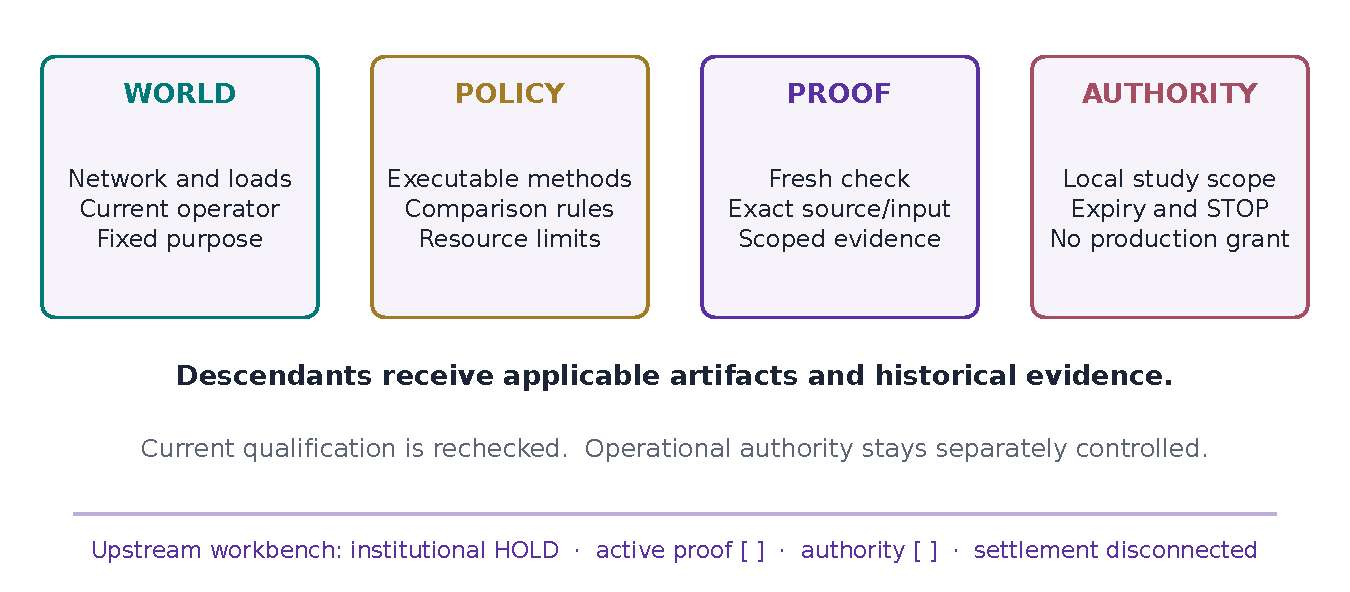
\includegraphics[width=\linewidth]{figures/proof-authority-boundary.pdf}
\caption{The four inspectable objects remain separate. A successor can inherit an applicable method and historical evidence. Its current output still needs a fresh check; institutional admission and operational authority are not inherited.}
\label{fig:authority}
\end{figure}

WORLD contains the supplied network and requirements. POLICY contains the fixed solver/construction policy
and resource rules. PROOF contains exact numerical checks, comparison records and their independence limits.
AUTHORITY contains only the bounded local study scope. The unchanged workbench pack records institutional
\artifact{HOLD}, empty active authority and disconnected settlement. A study-level product decision does not
edit that institutional status. An integrity hash identifies bytes; it is not an independent truth oracle.

\subsection{Jobs, Manager, Fleet and applicable token utility}

The actual inspected four-repository interfaces and five Alpha contract source identities are retained in the
audit manifests \citep{alphaContracts,alphaCoordination}. The workbench's existing Jobs compiler emits unfunded
bounded drafts. Jobs' inspected receiver uses AGIALPHA18; Manager's distinct receiver uses USDC6. Fleet's
control interface remains subject to its original source/review/action restrictions. None is invoked as a
numerical executor or settlement service by this experiment.

\begin{table}[ht]\centering\small
\begin{tabularx}{\linewidth}{L{32mm}Y}
\toprule
Inspected contract & Relevant function and scope \\
\midrule
AscensionAccess & \artifact{register}, \artifact{owns}, \artifact{setAdmission}, \artifact{eligible}: roles and expiring admission; no numerical proof. \\
NovaSeed & \artifact{seal}, \artifact{plan}, \artifact{creatorOf}: commitments and parent identity; no inherited current authority. \\
AscensionRiskOracle & \artifact{lockForJob}, \artifact{openReview}, \artifact{attest}, \artifact{green}: staked review/capacity; not an independent mathematical checker. \\
AscensionJobMarket & \artifact{post}, \artifact{award}, \artifact{submit}, \artifact{validate}, \artifact{timeout}: bounded funded work and settlement if separately authorized. \\
AscensionMark & \artifact{open}, \artifact{buy}, \artifact{route}, \artifact{collect}, \artifact{close}: funding/routing and closure; token movement is not productive value. \\
\bottomrule
\end{tabularx}
\caption{Source inspection only. No deployed address, chain state, local EVM execution, funded draft, signed transaction or live settlement is established. No contract call is needed to solve these missions.}
\end{table}

Practical \$AGIALPHA utility would require separately authorized funded work and the applicable contract
conditions. It is not inferred from this experiment's branding, token scarcity or price. The new edition
preserves previous URLs and awaits its own exact-source review and publication process. Draft preparation,
review, merge, public release and served-file verification are reported separately; original Harness/Fleet
holds and the existing publication owner's sequencing remain binding.
